\documentclass{article}
\usepackage{amsmath,enumitem,fullpage,graphicx,listings,float,sidecap,setspace,xcolor,wrapfig,booktabs,multirow,subcaption,array,minted,hyperref,xepersian,bidi,svg}
%compile with xelatex+shell+escape
\newcolumntype{C}[1]{>{\centering\arraybackslash}m{#1}}

\definecolor{lg}{HTML}{F4F3F3}
\setlength{\fboxsep}{10pt}
\usemintedstyle{borland}
\hypersetup{
    colorlinks=true,
    linkcolor=blue,
    citecolor=green,
    filecolor=magenta,
    urlcolor=cyan
}
\fontsize{14pt}{16pt}\selectfont
\setlatintextfont{IRNazanin.ttf}
\settextfont{IRNazanin.ttf}

\begin{document}
\begin{titlepage}
    \centering
    \begin{figure}[ht]
        \centering
        
\includegraphics[width=0.5\textwidth]{iust.png}
    \end{figure}
    \vspace{1cm}
    {\scshape\Huge \textbf{دانشکده مهندسی کامپیوتر} \par}
    \vspace{1cm}
    {\huge\bfseries پروژه ایریدیوم  \par}
    \vspace{1cm}
    {\Large امنیت سیستم‌های کامپیوتری \par}
    \vspace{1cm}
	{\LARGE  مدرس: دکتر ابوالفضل دیانت\par}
    \vspace{1cm}
    {\LARGE  محمدحسین عباسپور، فرزان رحمانی \par}
    \vspace{1cm}
    {\LARGE شماره دانشجویی: ۹۹۵۲۱۴۳۳، ۹۹۵۲۱۲۷1 \par}
    \vspace{1.22cm}
    {\large نیم سال دوم \par}
    {\large سال تحصیلی ۱۴۰۳-۱۴۰۲ \par}
\end{titlepage}
\newpage
\doublespacing
\singlespacing
\newpage
\setstretch{1.5}
\section {مقدمه}
\leavevmode 
\\
در سال ۲۰۱۶ بدافزاری به نام Mirai دست به آلوده کردن هزاران دستگاه با ارسال درخواست DNS به سرور و مختل کردن آن، باعث از بین رفتن دسترسی بسیاری از وبسایت‌های معروف جهان شد. در این پروژه قصد داریم که یک شبیه‌ساز از این بدافزار بوجود بیاوریم.
\\
\section {توضیح پروژه}
\leavevmode
\\
در این پروژه ما باید شبکه را اسکن کنیم و به دنبال پورت‌های باز شبکه بگردیم و در آنهایی که برای سرویس ssh میباشند، با آزمایش چندین رمز به این سیستم‌ها نفوذ کرده و بدافزاری را روی آنها بارگذاری کنیم تا اطلاعات مهم سیستم را جمع‌آوری کند. برای نفوذ از چند رمز معروف مانند admin استفاده کردیم و اگر رمز آن سیستم جزو این پسور‌های معروف نباشد نمیتوانیم وارد سیستم شویم. دقیقا مشابه روش .Mirai
\\
\section{ساختار پروژه}
\leavevmode
\\
برای پیاده‌سازی این پروژه از docker استفاده کردیم. در ابتدا به کمک داکر یک شبکه داکر ایجاد کردیم و داخل آن تعداد container ساختیم. در ابتدا باید برای هر سرویس یک image بسازیم:
\begin{itemize}
\item attacker-image
\item target-server-image
\item web-server-image
\end{itemize}
سپس بعد از اینکه تمام این سرویس‌ها را بالا آوردیم، حمله را انجام میدهیم.\\
\subsection{attacker-image}
\leavevmode 
\\
وظیفه این ماشین همانطور که از اسمش پیداست برای حمله به هدف میباشد. این ماشین بعد از بالا آمدن با استفاده از اسکریپت scan.sh اقدام به اسکن پورت‌های باز و شناسایی آنهایی که سرویس ssh بر روی آنها اجرا میشود میکند. این اسکریپت در یک محدوده از IP ها، تمام هاست‌های فعال را بررسی میکند که آیا پورت مدنظر را دارد یا نه. سپس آنها را ذخیره میکند. \\
در گام بعدی با استفاده از اسکریپت hack.sh شروع به حمله به تک تک پورت‌های ذخیره شده‌ی هاست‌ها میکند. برای حمله نیاز به تعدادی رمز داریم تا آنها را بر روی قربانی تست کنیم. این رمز‌ها داخل فایل user\_password.csv قرار دارند:
\begin{figure}[h]
\centering
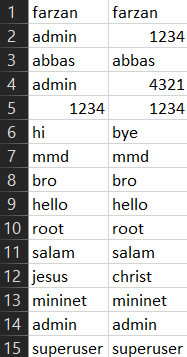
\includegraphics[width=0.18\textwidth]{images/csv.png}
\end{figure}
پس از تست کردن این رمزها، در صورتی که ارتباط با قربانی برقرار شد، بدافزار از وب‌سرور بر روی سرور قربانی آپلود میشود. \\
\subsection{target-server-image}
\leavevmode
\\
این سرورها، سرورهای قربانی هستند که بدافزار بر روی آنها قرار میگیرد. در اینجا ۵ عدد سرور را با استفاده از داکر بالا می‌آوریم.\\
\subsection{web-server-image}
\leavevmode
\\
این وب سرور ساده را با استفاده از django ایجاد کردیم. وظیفه این ماشین دانلود بدافزار، ارسال اطلاعات قربانی، ذخیره اطلاعات در یک دیتابیس و یک رابط کاربری برای مشاهده اطلاعات میباشد. در اینجا چون خیلی پروژه سنگینی نبود از دیتابیس پیش‌فرض django یعنی sqlite استفاده کردیم. وظایفی که ذکر شد توسط اسکریپتی به نام infogather.sh انجام میشود. \\
نمونه‌ای از اطلاعات ذخیره‌شده در دیتابیس در شکل زیر قابل مشاهده است:
\begin{figure}[h]
\centering
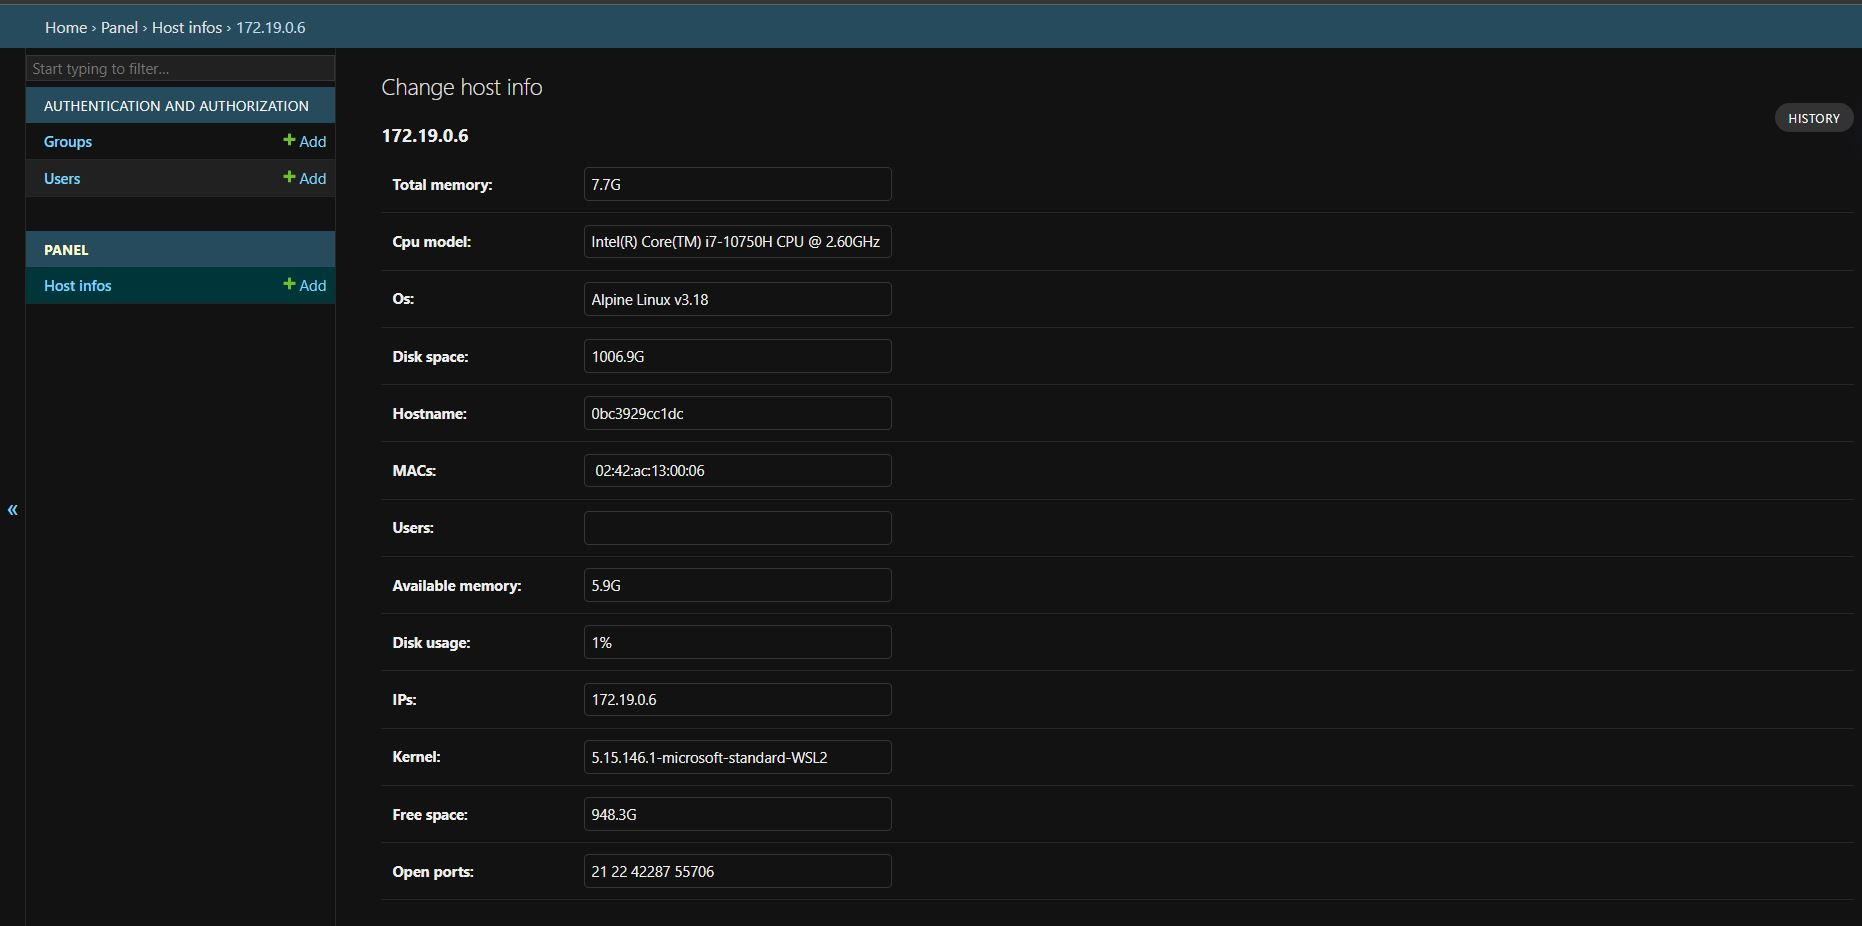
\includegraphics[width=1.0\textwidth]{images/victim.jpg}
\end{figure}\\
\newpage
\section{اجرای پروژه}
\leavevmode
\\
برای اجرای پروژه در ابتدا باید تمام image ها را ایجاد کنیم. برای این کار از اسکریپت build\_images.sh استفاده میکنیم.
\begin{figure}[ht]
\centering
\includegraphics[width=0.9\textwidth]{images/build\_images.jpg}
\end{figure}

 در مرحله بعد باید شبکه داکر را بوجود بیاوریم. برای این کار از اسکریپت setup\_sim.sh استفاده میکنیم. این اسکریپت شبکه داکر را ایجاد میکند سپس image های:
\begin{itemize}
\item attacker-server-image
\item target-server-image
\item web-server-image
\end{itemize} 
\begin{figure}[ht]
\centering
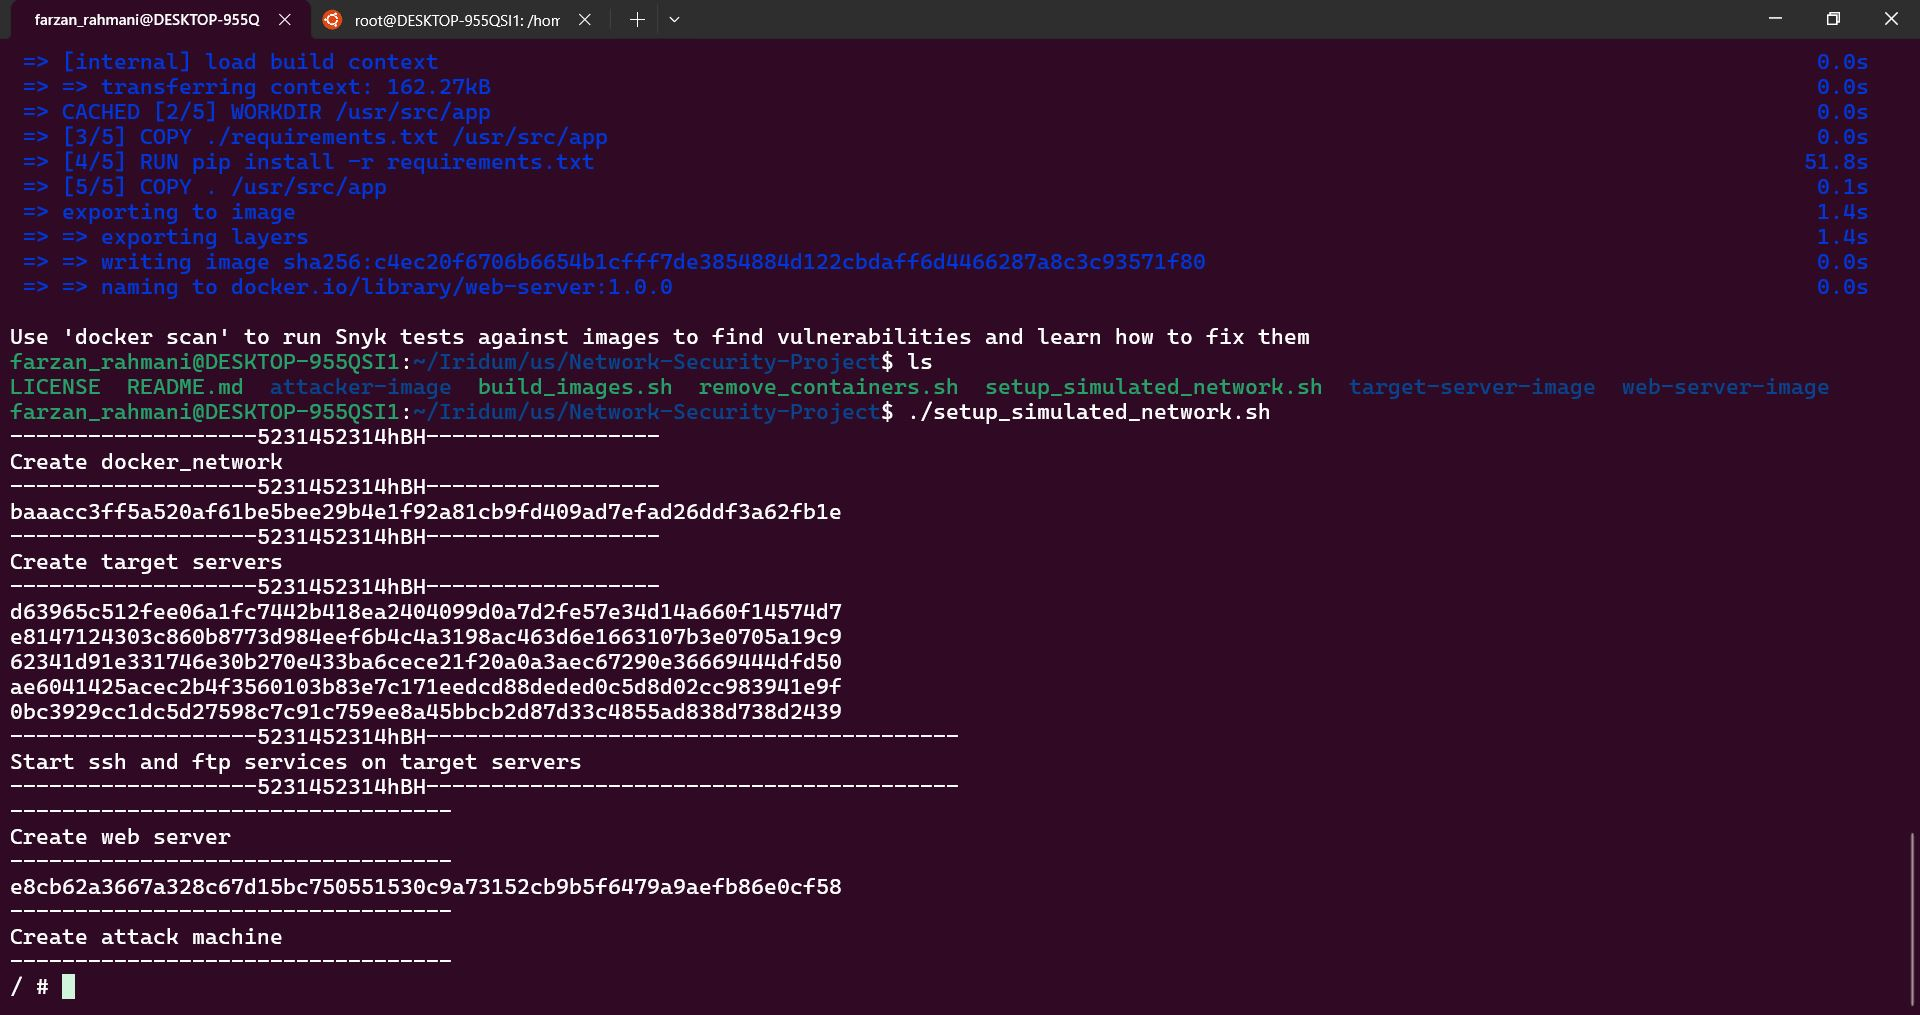
\includegraphics[width=0.9\textwidth]{images/setup.jpg}
\end{figure}
را اجرا میکند. 
\newpage
ابتدا با استفاده از دستور \lr{docker network inspect} آدرس شبکه داکر را پیدا میکنیم:
\begin{figure}[ht]
\centering
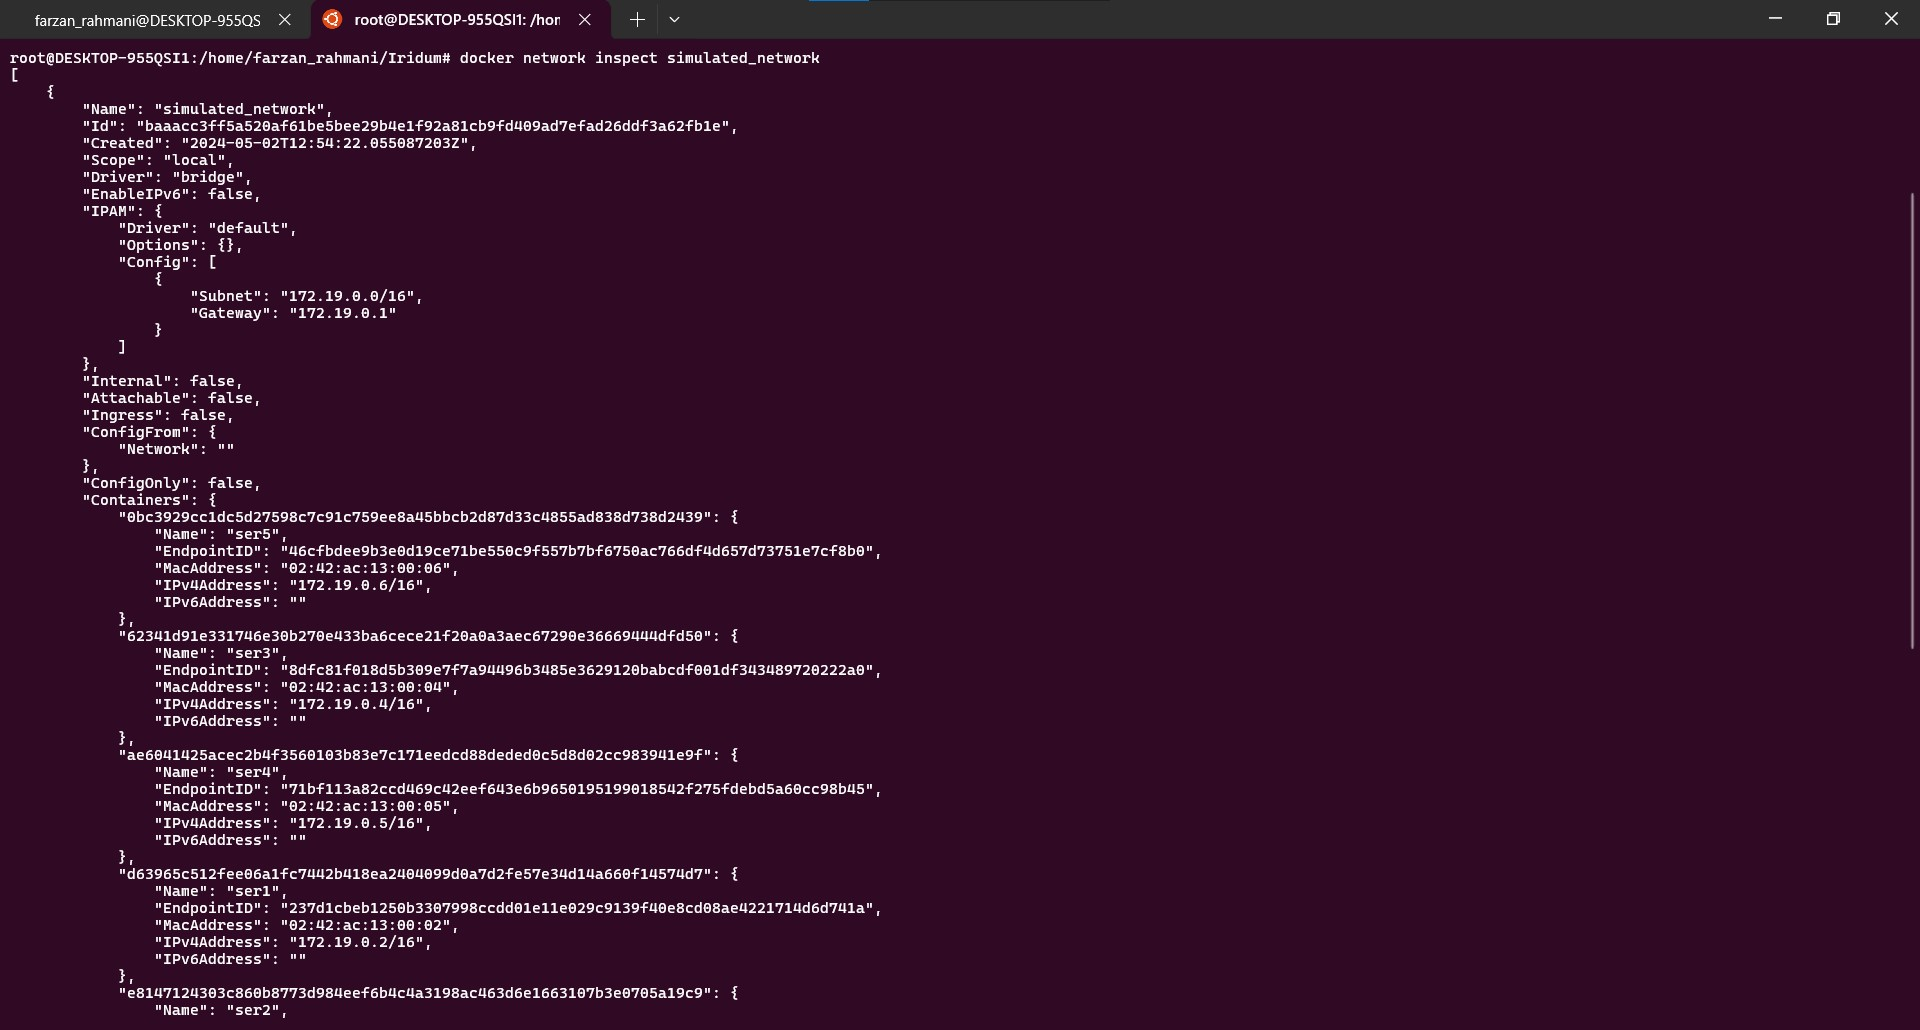
\includegraphics[width=0.9\textwidth]{images/inspect.jpg}
\end{figure}
\newpage
سپس اسکریپت scan.sh اجرا میکنیم محدوده مدنظر برای اسکن را به آن میدهیم. پس از اتمام، پورت‌های باز داخل فایل open\_ports.csv ذخیره میشوند: 
\begin{figure}[h]
\centering
\includegraphics[width=0.7\textwidth]{images/open\_ports.jpg}
\end{figure}


در مرحله بعد اسکریپت hack.sh را اجرا میکنیم:
\begin{figure}[ht]
\centering
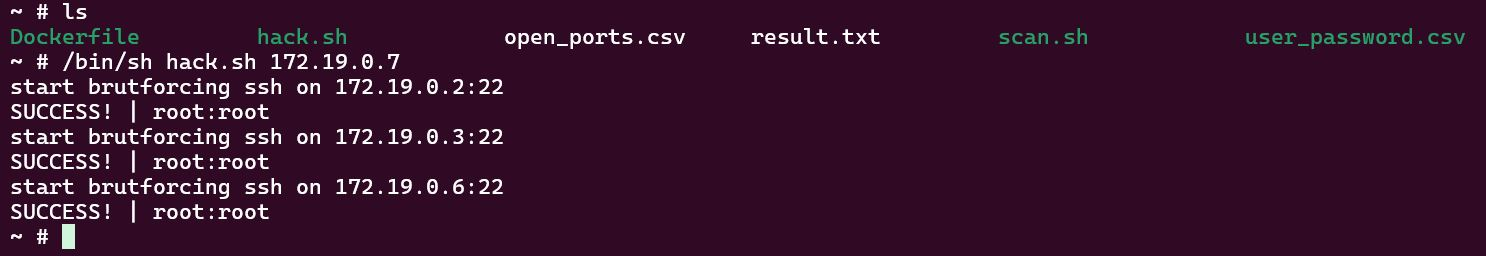
\includegraphics[width=0.7\textwidth]{images/hack.jpg}
\end{figure}
\newpage
اطلاعات ارسا‌شده توسط سرورهای قربانی در دیتابیس ذخیره می‌شوند:
\begin{figure}[ht]
\centering
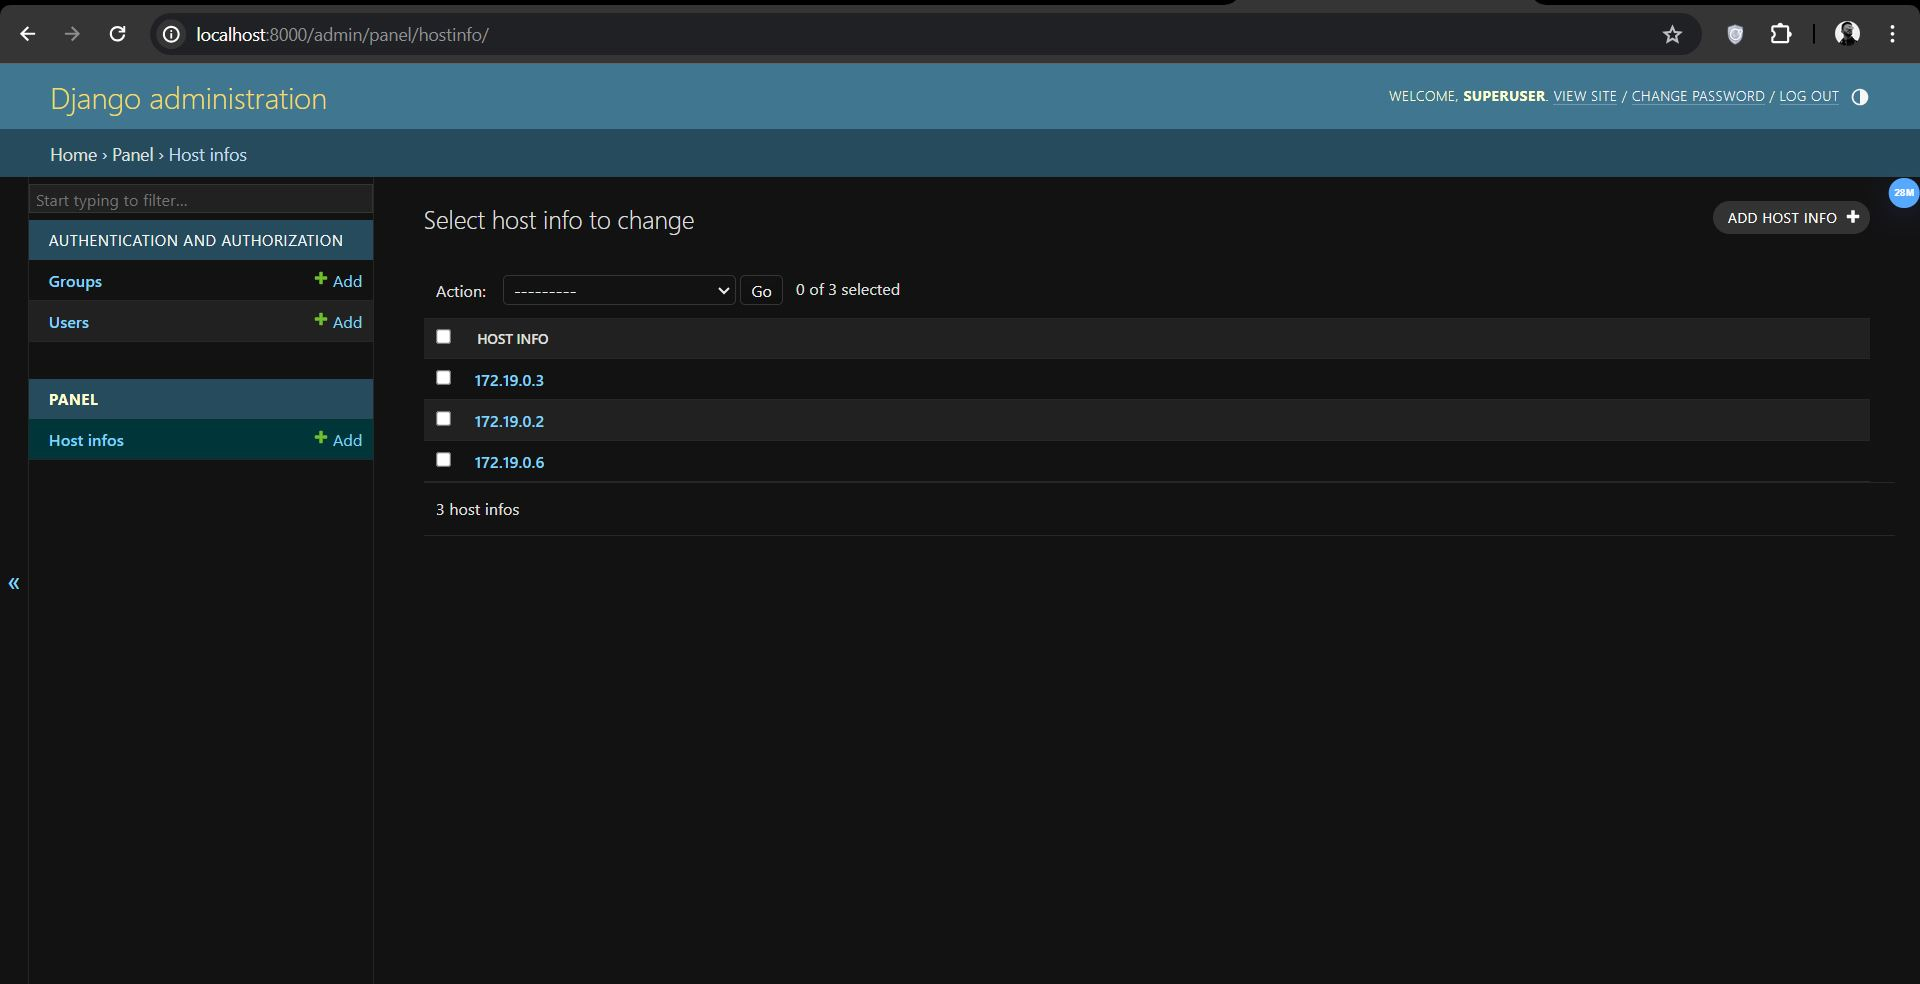
\includegraphics[width=0.7\textwidth]{images/ws.jpg}
\end{figure}


در آخر برای متوقف کردن و حذف شبکه داکر و container ها از اسکریپت remove\_containers.sh استفاده میکنیم.
\end{document}
